\documentclass[a4paper]{extarticle}
\usepackage[utf8]{inputenc}
\usepackage[a4paper, margin=1in]{geometry}

\usepackage{amssymb}
\usepackage{amsmath}
\usepackage{enumitem}
\usepackage{tcolorbox}
\usepackage{fancyhdr}
\usepackage{graphicx}
\usepackage{float}

\setlength{\parindent}{0em}
\setlength{\parskip}{0.4em}

\definecolor{theoremblue}{RGB}{1, 73, 124}
\definecolor{corollaryblue}{RGB}{70, 143, 175}
\definecolor{exampleblue}{RGB}{137, 194, 217}

\newtcolorbox{tbox}{colback=theoremblue!20,colframe=theoremblue,
boxrule=0pt,arc=0pt,boxsep=2pt,left=2pt,right=2pt,leftrule=2pt}

\newtcolorbox{cbox}{colback=corollaryblue!20,colframe=corollaryblue,
boxrule=0pt,arc=0pt,boxsep=2pt,left=2pt,right=2pt,leftrule=2pt}

\newtcolorbox{ebox}{colback=exampleblue!20,colframe=exampleblue,
boxrule=0pt,arc=0pt,boxsep=2pt,left=2pt,right=2pt,leftrule=2pt}

\title{FMFP - Lecture Notes Week 5}
\author{Ruben Schenk, ruben.schenk@inf.ethz.ch}
\date{\today}

\pagestyle{fancy}
\fancyhf{}
\rhead{ruben.schenk@inf.ethz.ch}
\rfoot{Page \thepage}
\lhead{FMFP - Lecture Notes Week 5}

\begin{document}

\maketitle
\newpage

\section{Typing}

\subsection{Overview}

\textbf{Type checking} should prevent "dangerous expressions", such as \verb|2 + True|, \verb|[2] : [3]|, etc. Dangerous expressions lead to \textit{runtime errors.}

The objectives for a type checker are as follows:

\begin{itemize}
    \item Quick, decidable, static analysis
    \item Permit as much generality / re-usability as possible
    \item Prevent runtime errors
\end{itemize}

\subsection{Mini-Haskell}

\subsubsection{Syntax}

Programs are \textbf{terms} (for now, let variables \(\mathcal{V}\) and integers \(\mathcal{Z}\) be given):

\begin{align*}
    t \, ::= \, &\mathcal{V} \, | \, (\lambda x.t) \, | \, (t_1 \, t_2) \, | \\
    &True \, | \, False \, | \, (\text{iszero } t) \, | \\
    & \mathcal{Z} \, | \, (t_1 + t_2) \, | \, (t_1 * t_2) \, | \, (\text{if } t_0 \text{ then } t_1 \text{ else } t_2) \, | \\
    &(t_1, \, t_2) \, | \, (\text{fst } t) \, | \, (\text{snd } t)
\end{align*}

The core of Mini-Haskell is \(\lambda\)-calculus: variables, abstractions, and applications. Additional syntax and types can be easily added, e.g. \verb|&&|, \verb|Strings|, etc.

We employ some syntactic sugar, like omitting parenthesis (e.g. \verb|x y z| instead of \verb|((x y) z)|).

\subsubsection{Typing}

We consider \textbf{types}, given \(\mathcal{V}_{\tau}\) is a set of variables like \(a\), \(b\), etc., such that

\[
    \tau \, ::= \, \mathcal{V}_{\tau} \, | \, Bool \, | \, Int \, | \, (\tau, \, \tau) \, | \, (\tau \to \tau)
\]

The type system notation is based on \textbf{typing judgements} of the following form:

\[
    \Gamma \vdash t :: \tau,
\]

where:

\begin{itemize}
    \item \(\Gamma\) is a set of bindings \(x_i : \tau_i\), mapping variables to types. Intuitively, \(\Gamma\) represents a kind of typing "symbol table".
    \item \(t\) is a \textit{term}
    \item \(\tau\) is a \textit{type}
\end{itemize}

\begin{ebox}
    \textbf{Example:}
    \[
        x : int \vdash x + 2 :: Int
    \]
    \[
        x : Int, \, f : Bool \to Bool \nvdash f \, x :: Bool        
    \]
\end{ebox}

\subsubsection{Proof System}

\textbf{Proof rules} are formulated in terms of type judgements \(J\):

\[
    \frac{J_1 \quad \cdots \quad J-n}{J}
\]

For example, one rule could be, given \(op \in \{+, \, *\}\), the \(BinOp\) rule:

\[
    \frac{\Gamma \vdash t_1 :: Int \quad \Gamma \vdash t_2 :: Int}{\Gamma \vdash (t_1 \, op \, t_2) :: Int}
\]

\subsubsection{Rules For Core \(\lambda\)-Calculus}

We introduce the following rules for the core \(\lambda\)-calculus:

\paragraph{Axiom}:

\begin{figure}[H]
    
\includegraphics[width=6cm]{../images/FMFP_Fig5-1}
    \centering
\end{figure}

\paragraph{Abstraction} (\(x \notin \Gamma\)):

\begin{figure}[H]
    
\includegraphics[width=6cm]{../images/FMFP_Fig5-2}
    \centering
\end{figure}

\paragraph{Application}:

\begin{figure}[H]
    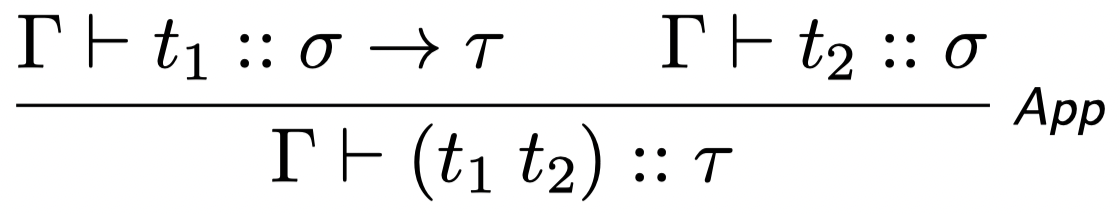
\includegraphics[width=6cm]{../images/FMFP_Fig5-3}
    \centering
\end{figure}

\subsubsection{Further Typing Rules}

\begin{figure}[H]
    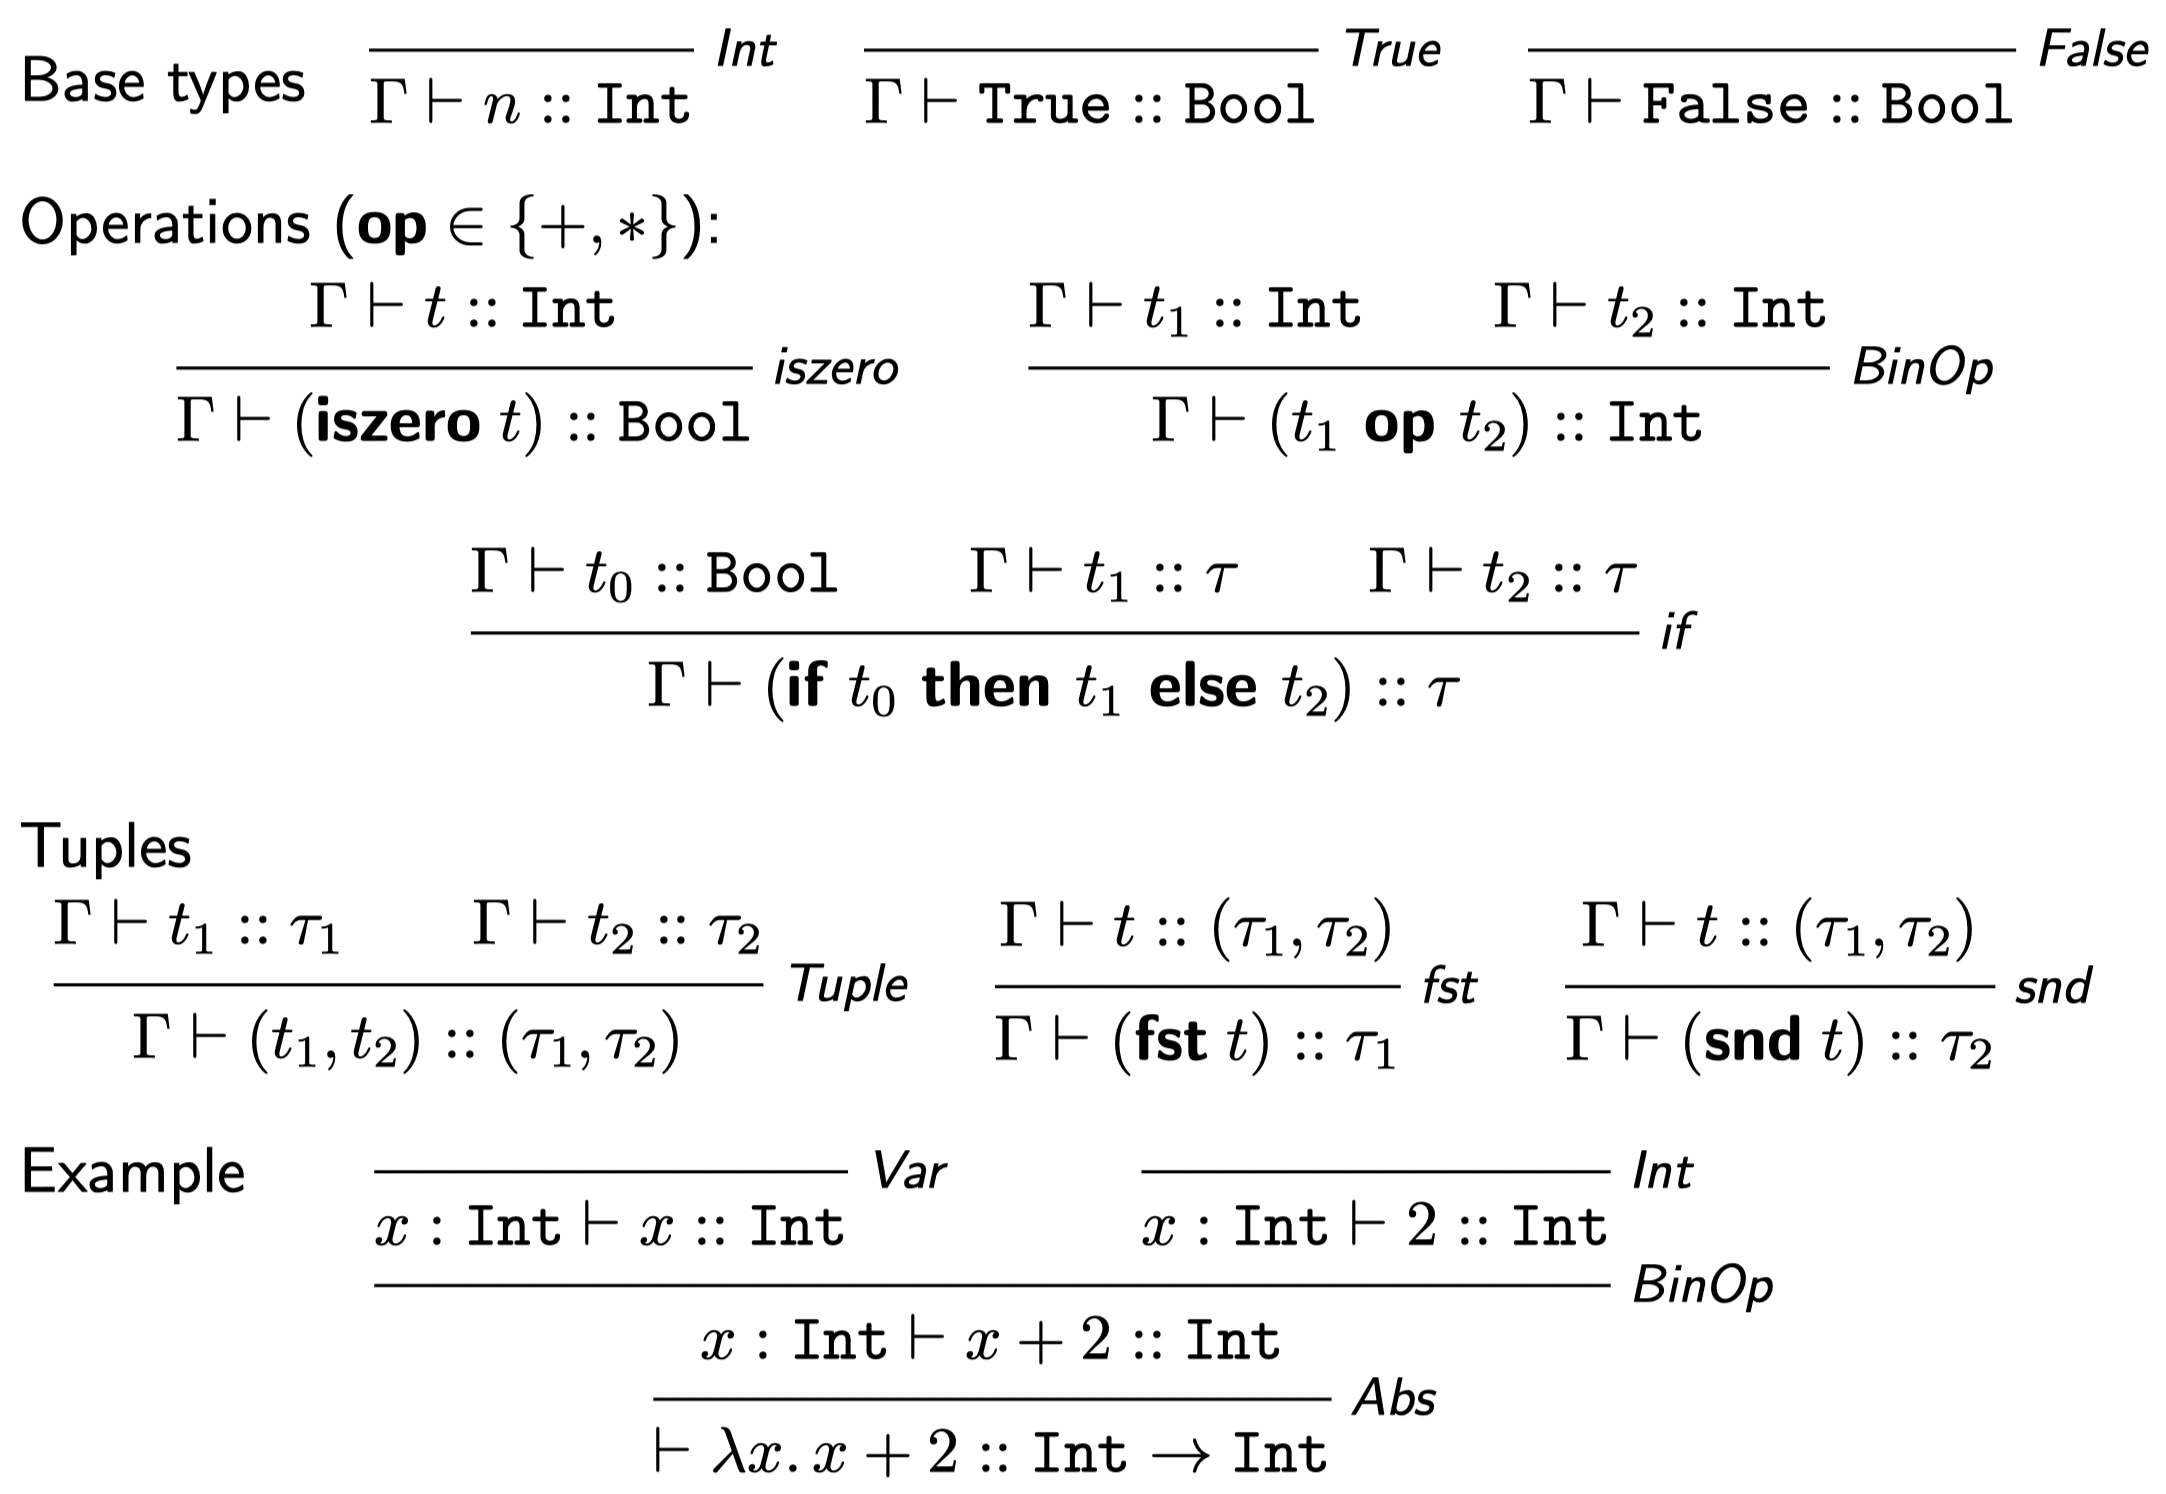
\includegraphics[width=15cm]{../images/FMFP_Fig5-4}
    \centering
\end{figure}

\subsection{Type Inference}

Syntax-directed typing rules specify an algorithm for computing the type of expressions:

\begin{enumerate}
    \item Start with judgement \(\vdash t :: \tau_0\) with type variable \(\tau_0\).
    \item Build the derivation tree bottom-up by applying the available rules. Introduce fresh type variables and collect constraints if needed.
    \item Solve constraints to get possible types.
\end{enumerate}

\begin{ebox}
    \textbf{Example:}

    \begin{figure}[H]
        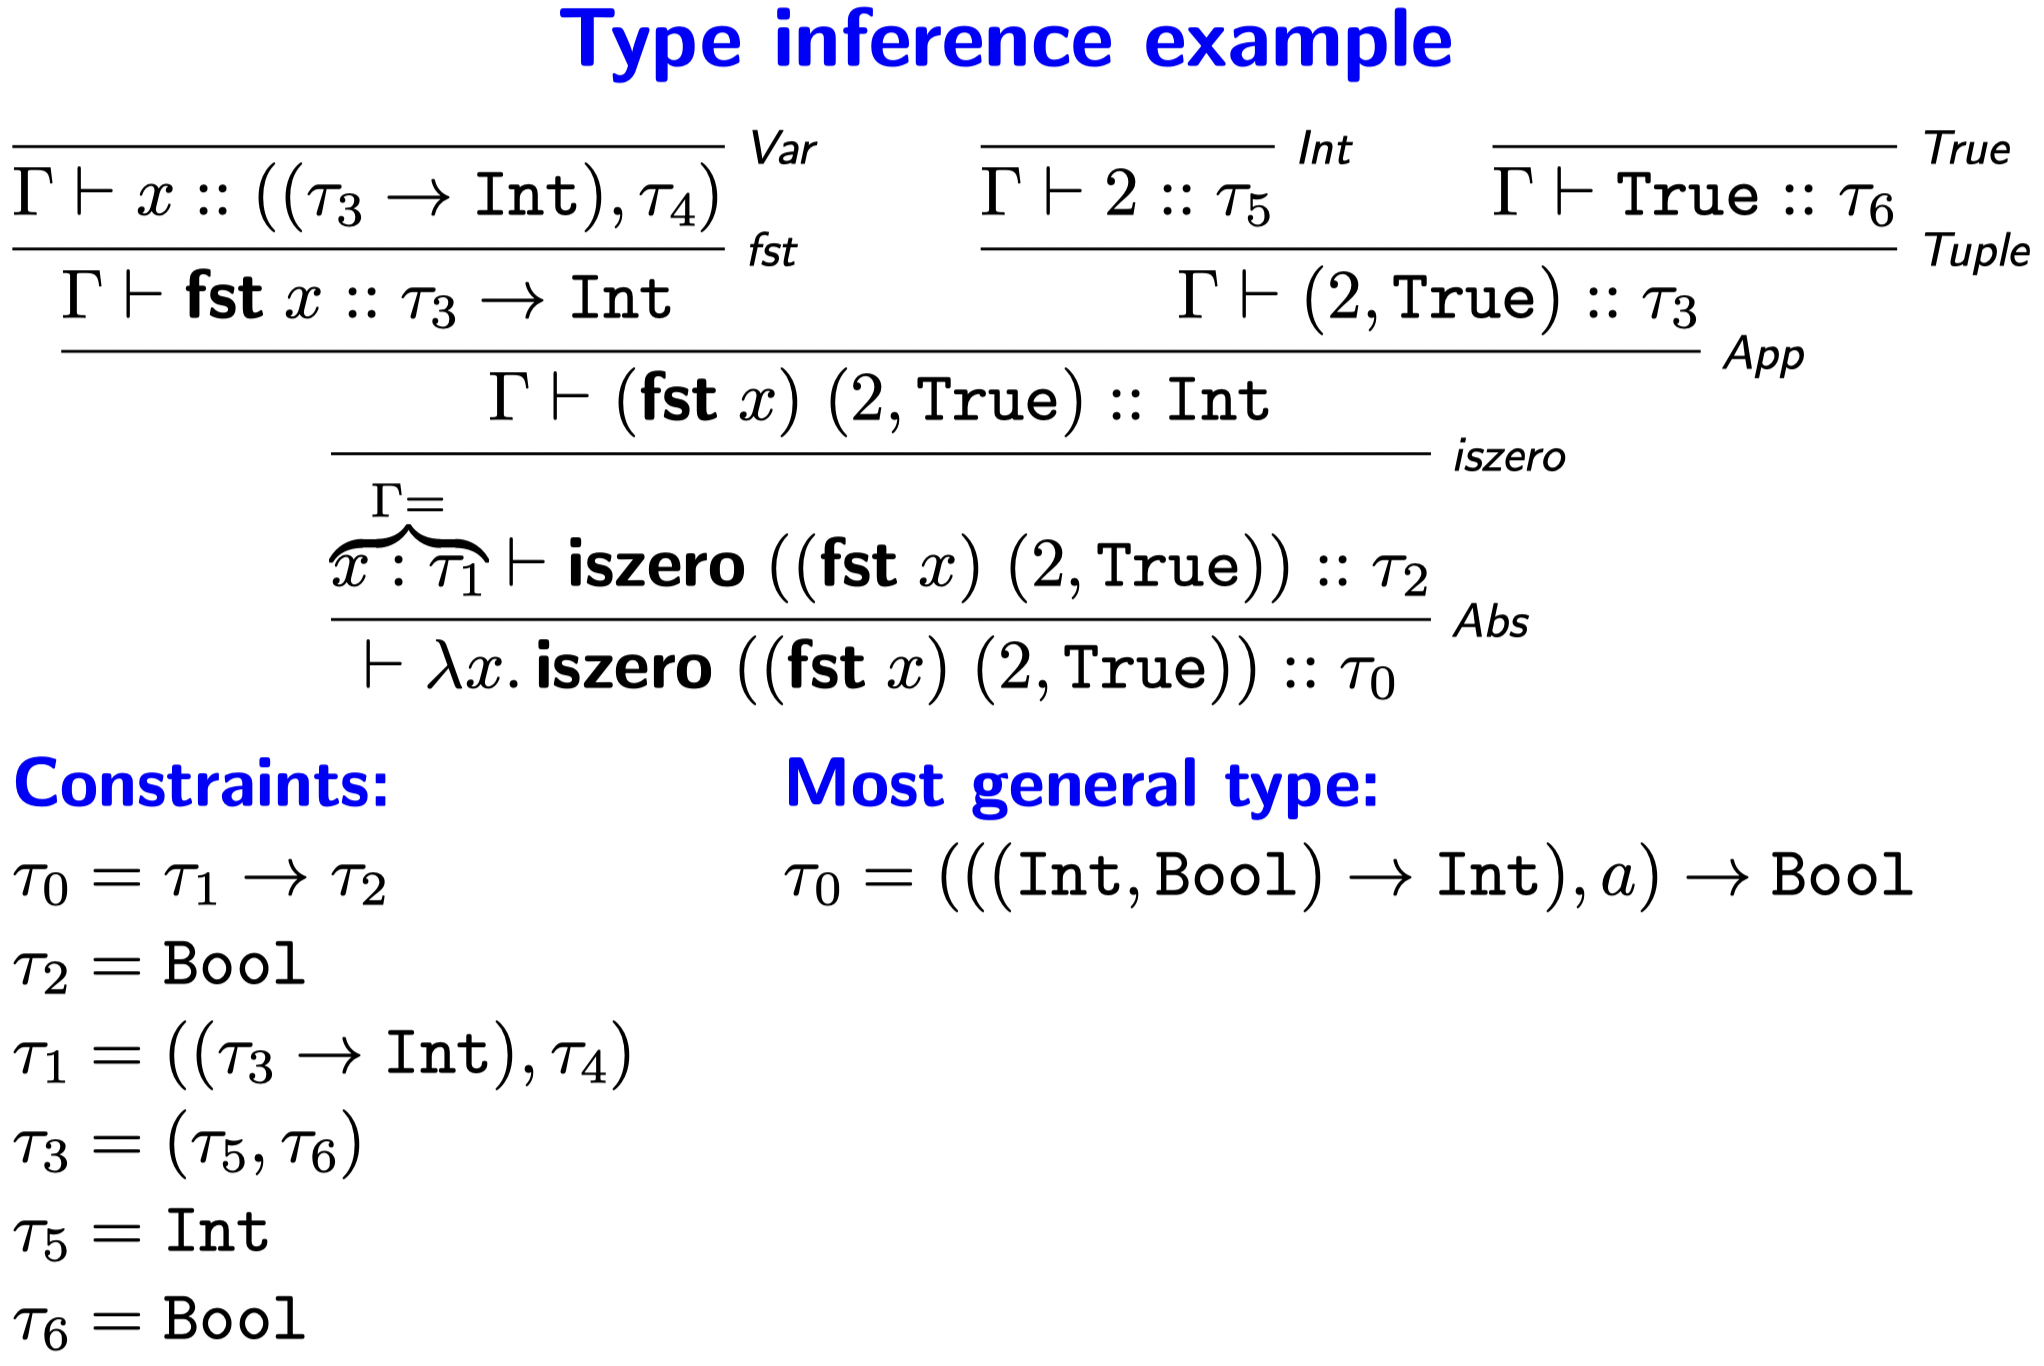
\includegraphics[width=12cm]{../images/FMFP_Fig5-5}
        \centering
    \end{figure}
\end{ebox}

\subsection{Type Classes}

\subsubsection{Monomorphic vs. Polymorphic}

We can distinguish between monomorphic and polymorphic functions. Some \textbf{monomorphic} functions:

\begin{verbatim}
    xor x y = (x || y) && (not (x && y))

    ? :type xor
    xor :: Bool -> Bool -> Bool
\end{verbatim}

Others are \textbf{polymorphic:}

\begin{verbatim}
    []     ++ ys = ys
    (x:xs) ++ ys = x : (xs ++ ys)

    ? :type (++)
    (++) :: [a] -> [a] -> [a]
\end{verbatim}

\subsubsection{Type Classes - The Middle Way}

Type classes allow for polymorphism to be restricted using class constraints. Example:

\begin{verbatim}
    allEqual :: Eq a => a -> a -> a -> Bool
    allEqual x y z = (x == y) && (y == z)
\end{verbatim}

Functions for precisely those types \(a\) that belong to the \textbf{class} \(Eq\). For example, the definition for the \(Eq\) class is given as follows:

\begin{verbatim}
    class Eq a where
        (==) :: a -> a -> Bool
        (/=) :: a -> a -> Bool

        x /= y = not (x == y)
\end{verbatim}

The definition includes:

\begin{enumerate}
    \item Class name: \(Eq\)
    \item Signature: List of function names and types
    \item Default implementations (optional): Can be overwritten later
\end{enumerate}

Elements of a class are called \textbf{instances.} \verb|instance| builds instances by "interpreting" signature functions:

\begin{verbatim}
    instance Eq Bool where
        True  == True  = True
        False == False = True
        _     == _     = False
\end{verbatim}

\end{document}